\item[4.~定理.] \emph{限界曲線は、円と等距離曲線との間の極限の曲線である。それは半径が無限に大きい円とも、基線が無限に遠い等距離曲線ともみなせる。}

\begin{figure}[h]
\centering
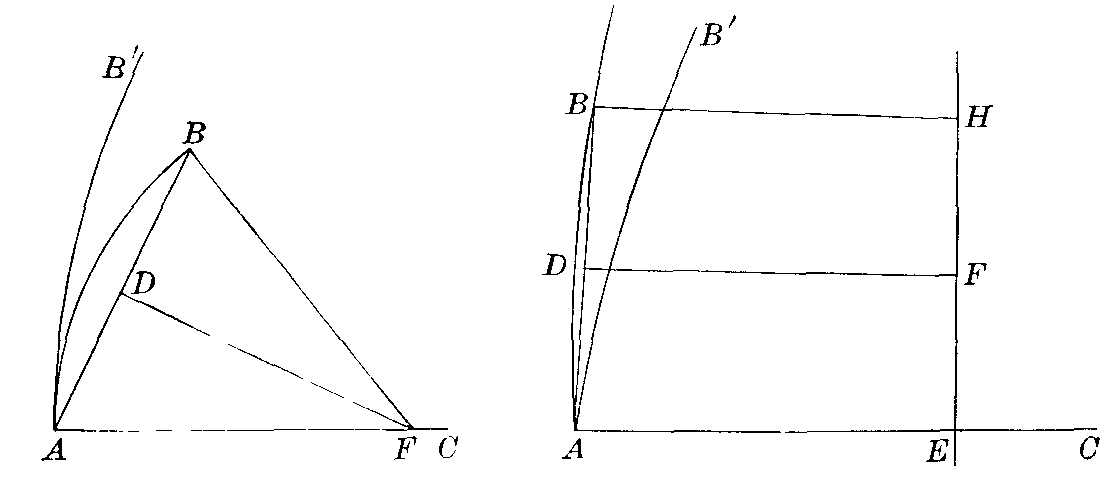
\includegraphics[width=80mm]{fig51.png}
\end{figure}

\textbf{証明.} 与えられた長さの線 $AB = 2a$ をとり、固定した線 $AC$ と角 $A$ をなすものとする。$B$ に角 $A$ に等しい別の角をつくり、$AB$ の中点 $D$ で $AB$ に垂線を引く。

$A$ での角が十分に小さければ、$AB$ を底辺とし、頂点が $AC$ 上の点 $F$ にある二等辺三角形ができる。$F$ を中心として、点 $A$ と $B$ を通る円を描くことができる。そこで $A$ での角を徐々に増し、図の他の部分は作図を保つように変化させる。$F$ は限りなく遠ざかり、$A = \Pi(a)$ となったとき、三本の線 $AF$、$BF$、$DF$ は平行になり、$B$ は、$AC$ を軸とする限界曲線 $AB'$ 上の点になる。

一方、$A$ での角を鋭角にとるが $\Pi(a)$ より大きくとれば、点 $A$ と $B$ を通る等距離曲線の基線 $EH$ に垂直な三本の線 $AE$、$BH$、$DF$ ができる。そこで角 $A$ を徐々に減らし、図の他の部分は作図を保つように変化させる。三つの直角をもち、第四の角 $A$ が減少する四角形 $ADFE$ は、面積が増加しなければならない。これと同じ動きは、$AD$ と $DF$ が平面上で固定されたまま、$AE$ が $A$ のまわりに回転して角 $A$ が減少すると考えても得られる。このように、四角形の面積が増加しうる唯一の方法は、$EH$ が $AC$ に沿って遠ざかり、$A$ からますます遠くなることである。$A$ が $\Pi (a)$ に等しくなるとき、$BH$ と $DF$ は $AC$ に平行になり、$B$ は限界曲線 $AB'$ の上に落ちる。
\end{description}

円の半径を軸と呼ぶことにすると、円、限界曲線、等距離曲線には共通の性質が多いことがわかる。

任意の弦の中点に立てた垂線は軸である。とくに、接線は、その接点から引いた軸に垂直である。これらは、それぞれ、一点を通る線の系、平行線の系、与えられた線への垂線の系を直角に切る曲線である。

同じ軸の組をもつこれらの曲線の二つは、これらの軸のすべてに等しい長さを切り取り、そのような二つの曲線上の対応する弧の比は、軸の分け方だけに依存する定数である。

三点がこれらの曲線の一つを定める。すなわち、一直線上にない任意の三点を通って、円か、限界曲線か、等距離曲線のいずれかである曲線を引くことができ、任意の三点を通る曲線はただ一つしか引けない。任意の三角形は、これらの曲線のただ一つに内接させることができる。

これらの曲線の各々は、それ自身の上を動かすことができ、また任意の軸のまわりに $180^\circ$ 回転させてそれ自身に重ねることができる。

\emph{限界面}あるいはオリスフィアとは、限界曲線をその軸の一つのまわりに回転させて生じる曲面である。

\begin{description}
\item[5.~定理.] \emph{限界面の軸に平行な任意の線を軸とみなすことができる。}

\begin{figure}[h]
\centering
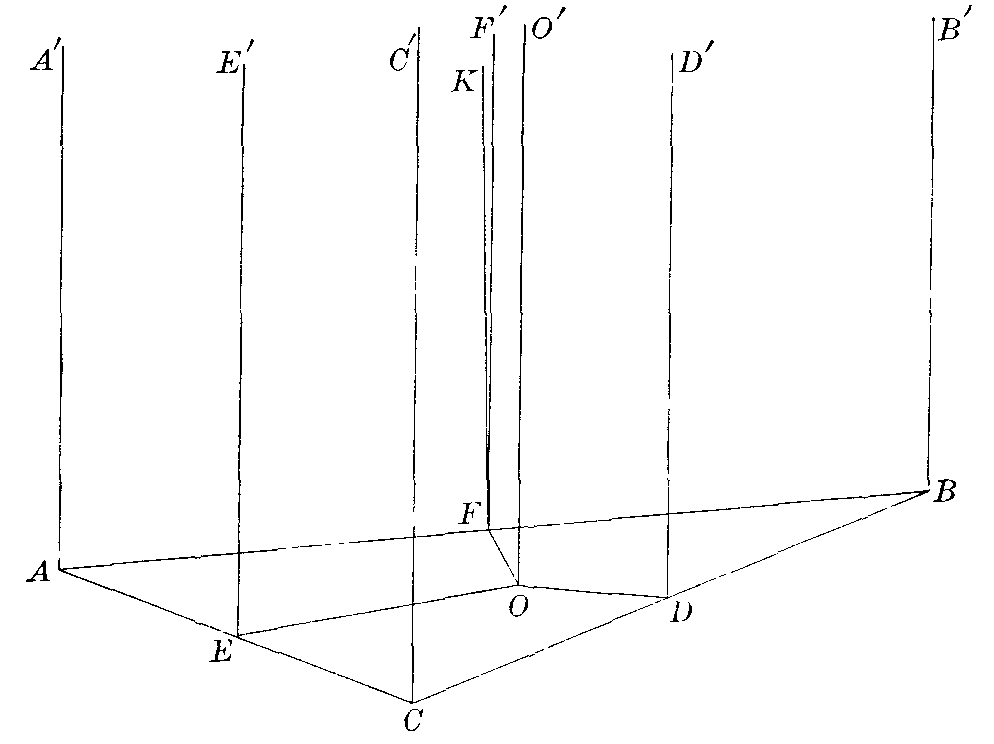
\includegraphics[width=80mm]{fig52.png}
\end{figure}

\textbf{$AA'$} を、曲面と $A$ で出会う軸とし、$BB'$ を曲面の任意の他の点 $B$ を通る軸に平行な線とする。$BB'$ を軸とみなせることを証明する。

\textbf{証明.} $C$ を曲面上の第三の点とする。$C$ を通って $CC'$ を引き、平面三角形 $ABC$ の各辺の中点 $D$、$E$、$F$ を通って、すべて $AA'$ に平行な $DD'$、$EE'$、$FF'$ を引く。最後に、これらの線に平行で平面 $ABC$ に垂直な $OO'$ を引く。他の平行線の射影平面は、すべて $OO'$ を通る（I, 9 を見よ）。

$AA'$ は曲面の軸であるから、$EE'$ と $FF'$ は、それぞれ $AC$ と $AB$ に垂直である。$F$ で平面 $ABC$ に垂直に $FK$ を引く。それは射影平面 $OFF'$ に含まれる。$AB$ は $FF'$ と $FK$ に垂直であるから、この平面 $OFF'$ に、したがって $OF$ に垂直である。同様にして、$AC$ が $OE$ に垂直であることが証明される。したがって、$BC$ は $OD$ に垂直である（第I章, I, 5）。しかるに $OD$ は平面 $ABC$ と平面 $ODD'$ の交線である。ゆえに $BC$ はこの平面に、また $DD'$ に垂直である（第I章, II, 15）。

$DD'$ は $BB'$ に平行であるから、$BB'$ と $BC$ で定まる平面に含まれ、この平面内では、$BC$ にその中点で垂直な線はただ一本しか引けない。したがって、$BB'$ を通る任意の平面をとり、$B$ からこの平面と曲面との交わりの任意の他の点 $C$ へ弦を引くと、この平面内で $BC$ の中点に立てた $BC$ への垂線は $BB'$ に平行である。これは、断面が $BB'$ を軸とする限界曲線であり、曲面がそのような限界曲線を $BB'$ のまわりに回転させて生成できることを証明している。

ゆえに、$BB'$ は曲面の軸とみなせる。
\end{description}

限界面の軸を通る平面を\emph{主平面}という。すべての主平面は、曲面を限界曲線で切る。他の任意の平面は、曲面を円で切る。なぜなら、曲面は、その平面に垂直な軸を回転軸とする回転面とみなせるからである。この垂線を円の軸と呼び、それが曲面と出会う点を円の\emph{極}と呼ぶことができる。限界面上の円の極は、円のすべての点から等しい距離にある。ここで距離は、曲面上の限界線に沿って測る。

任意の二つの限界面を重ね合わせることができ、限界面は、任意の点を任意の他の点の位置へ、また最初の点を通る任意の限界曲線を第二の点を通る任意の限界曲線の位置へ、それ自身の上で動かすことができる。限界面は一定の曲率をもち、それはすべてのこれらの曲面で同じであると言ってよい。限界面上の図形は、形も大きさも変えずに動かすことができ、他の任意の限界面の上に置くことができる。

限界面上に幾何学を展開することができる。\emph{線}とは、曲面を主平面で切ってできる限界曲線を指す。二つの線のなす角は、曲面上にその線を切り出す二つの主平面の二面角に等しい。

\begin{description}
\item[6.~定理.] \emph{限界面上の幾何学は、通常のユークリッドの平面幾何学と同じである。}

\textbf{証明.} 同じ平行線の系を軸とする二つの限界面上では、対応する三角形は相似である。すなわち、対応する角は、それらを切り出す二面角と同じ大きさで等しく、対応する線は (2) により比例する。しかしこれらの図形を同じ曲面の上に置くことができるから、一つの限界面上に相似な三角形をもてる。こうして、三角形の辺を、その比も角も変えずに小さくできる。これは限りなく行える。なぜなら、二つの曲面上の対応する線の比は、それらの間の距離の関数 $e^{ax}$ で表されるから、$x$ を十分大きくとることにより望むだけ大きくできるからである。限界面上の図形は、その大きさを限りなく小さくするにつれて、ますます平面図形に似てゆくと仮定すれば、この曲面上の三角形は、角の和が二直角で、角と辺の関係がユークリッドの平面幾何学と同じである無限小の平面三角形の形に、ますます近づいてゆくことになる。したがって、われわれになじみのある平面三角法の公式はすべて、限界面上の三角形について成り立つ。

限界面上では「直角の仮説」が成り立つ。長方形をつくることができ、長方形の面積は底辺と高さの積に比例し、三角形の面積は、同じ底辺と高さをもつ長方形の面積の半分である。
\end{description}

\emph{等距離面}とは、等距離曲線をその軸の一つのまわりに回転させて生じる曲面である。それは、平面から与えられた垂直距離にある点の軌跡である。平面への任意の垂線を軸とみなすことができ、この曲面は、平面に垂直な線の系を直角に切る曲面である。この曲面は一定の曲率をもち、任意の位置でそれ自身に重なる。

\section{三角法の公式}

\begin{description}
\item[1.~] $ABC$ を平面の直角三角形とする。その平面に垂直に $AA'$ を立て、$AA'$ に平行に $BB'$ と $CC'$ を引く。$A$ を通り、これらの線を軸とする限界面を描き、限界面上の三角形 $AB''C''$ をつくる。また、点 $B$ のまわりに球面三角形をつくる。

\begin{figure}[h]
\centering
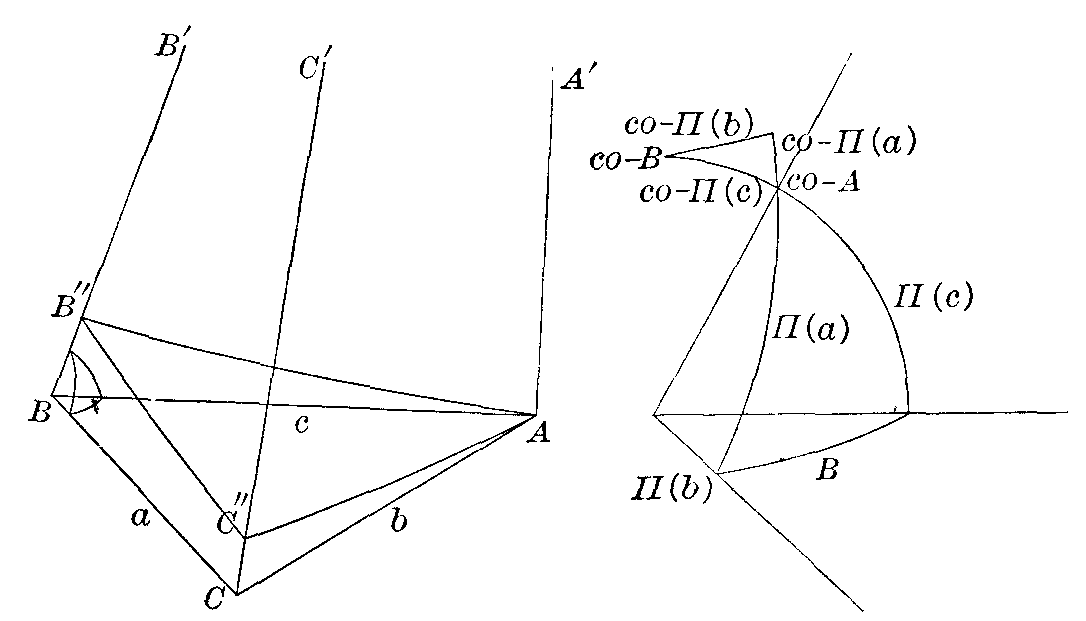
\includegraphics[width=80mm]{fig53.png}
\end{figure}

角 $A$ は、平面三角形と限界面上の三角形とで同じである。$AA'$ を通る平面は $ABC$ に垂直である。したがって、球面三角形は $c$ 上にある頂点に直角をもち、$CA$ に垂直な $BC$ は、$CC'$ と $AA'$ の平面に垂直である。ゆえに、平面 $BCC'$ は平面 $ACC'$ に垂直であり、辺が $BC$ である二面角の平面角は、角 $ACC'= \Pi (b)$ である。限界面上の三角形は $C''$ に直角をもつから、角 $B''$、あるいは同じことだが、辺が $BB'$ である二面角は、角 $A$ の余角である。

球面三角形では、直角に対する辺は $\Pi (a)$、直角をはさむ二辺は $\Pi (c)$ と $B$ であり、対する角は $\Pi (b)$ と $90^\circ-A$ である。

これらの量に球面直角三角形の三角法の公式を適用すると、ただちに平面直角三角形の辺と角を結ぶ関係が得られる。

$A$ の余角に等しい値をもつ角をはさむ二辺を、象限まで延長する。このようにして、直角に対する辺が $\Pi(c)$ の余角であり、直角をはさむ二辺が $\Pi(a)$ と $\Pi (b)$ の余角であり、それらに対する角が $B$ と $A$ の余角である球面直角三角形ができる。この三角形から、球面直角三角形の公式から平面三角形の公式へ移るための次の規則を導く。

\emph{二つの角（または二つの辺）を入れ替え、至るところで余関数を用い、辺については対応する平行角をとる。}

球面直角三角形の公式は、次のとおりである。
\begin{gather*}
\begin{aligned}
\sin A &= \frac{\sin a}{\sin c}. & \sin B &= \frac{\sin b}{\sin c}.\\
\cos A &= \frac{\tan b}{\tan c}. & \cos B &= \frac{\tan a}{\tan c}.\\
\tan A &= \frac{\tan a}{\sin b}. & \tan B &= \frac{\tan b}{\sin a}.\\
\sin A &= \frac{\cos B}{\cos b}. & \sin B &= \frac{\cos A}{\cos a}.
\end{aligned}\\
\begin{aligned}
\cos c &= \cos a \cdot \cos b \\
\cos c &= \cot A \cdot \cot B \\
\end{aligned}
\end{gather*}

これらから、前に与えた規則によって、平面直角三角形の次の公式を導く。
\begin{gather*}
  \begin{aligned}
    \cos B &= \frac{\cos\Pi(a)}{\cos\Pi(c)}. &
    \cos A &= \frac{\cos\Pi(b)}{\cos\Pi(c)}.\\
    \sin B &= \frac{\cot\Pi(b)}{\cot\Pi(c)}. &
    \sin A &= \frac{\cot\Pi(a)}{\cot\Pi(c)}.\\
    \cot B &= \frac{\cot\Pi(a)}{\cos\Pi(b)}. &
    \cot A &= \frac{\cot\Pi(b)}{\cos\Pi(a)}.\\
    \cos B &= \frac{\sin A}{\sin\Pi(b)}. &
    \cos A &= \frac{\sin B}{\sin\Pi(a)}.
  \end{aligned}\\
  \begin{aligned}
    \sin\Pi(c) &= \sin\Pi(a) \sin\Pi(b).\\
    \sin\Pi(c) &= \tan A \tan B.\footnotemark
  \end{aligned}
\end{gather*}
\footnotetext{直角三角形の各部分を、ネイピアの規則を適用できるように並べることができる。すなわち、配置は次のようになる。

\centering
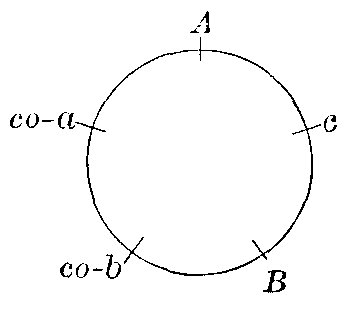
\includegraphics[width=30mm]{fig54.png}}

斜角の平面三角形の公式は、一つの頂点から対辺へ垂線を下ろし、二つの直角三角形をつくることによって得られる。

\item[2.~] 関係
\begin{equation*}
  \sin\Pi(a) = \frac{\sin B}{\cos A}
\end{equation*}
をとる。

\textbf{$p$}、$q$、$r$ を、前の証明の三角形 $AB''C''$ の辺とし、$p'$、$q'$、$r$ を、$B$ で平面 $ABC$ に接する限界面上に同じ方法でつくった三角形の対応する辺とする。

\begin{figure}[h]
\centering
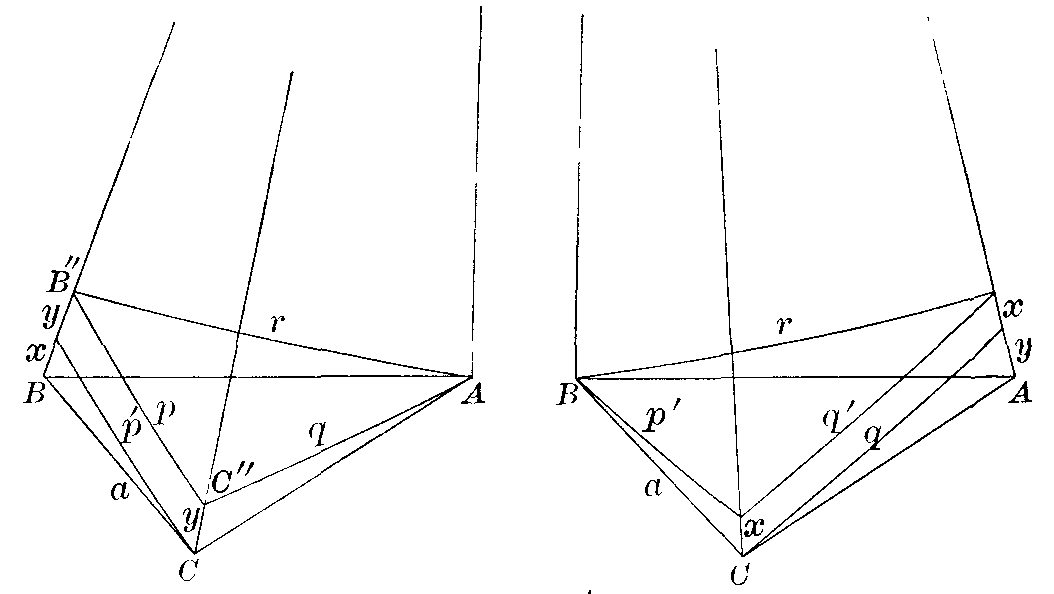
\includegraphics[width=80mm]{fig55.png}
\end{figure}

\begin{align*}
  \sin B &= \frac{q'}{r}, \\
  \cos A &= \frac{q}{r} . \\
  \therefore \sin \Pi(a) &= \frac{q'}{q} .
\end{align*}

\begin{figure}[h]
\centering
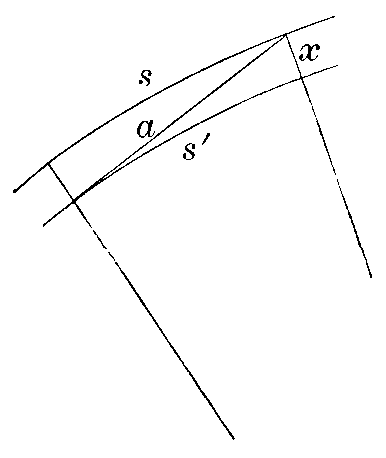
\includegraphics[width=35mm]{fig56.png}
\end{figure}

ここで $q$ と $q'$ は、同じ平行線の組を軸とする二つの限界曲線上の対応する弧であり、それらの間の距離 $x$ は、任意の長さ $a$ の接線の端点から限界曲線までの距離である。したがって、対応する弧について、
\begin{equation*}
  \frac{s'}{s} = \sin \Pi(a)
\end{equation*}
が成り立つ。

